\clearpage

   Um 2-dimensionale autonome DGL-Systeme zu veranschaulichen eignet sich das 
   Bild des Kopplungskonstanten-Flusses. Dabei "`fließt"' ein Anfangswert 
   $\alpha(t_0)$ entlang einer Trajektorie durch 
   den Phasenraum. Der Satz von Picard-Lindelöf stellt dabei sicher, dass 
   sich zwei Trajektorien nicht schneiden. Ein Flussdiagramm wie in Abbildung 
   \ref{beta_allgemein:fig:fluss_beispiel} zeigt das Verhalten von $\alpha(t)$ 
   indem das Geschwindigkeitsfeld $\beta$ durch Pfeile im Phasenraum 
   dargestellt wird. In dieser Arbeit zeigen die Pfeile stets in Richtung 
   steigender Energie. An dem Flussdiagramm \ref{beta_allgemein:fig:fluss_beispiel} 
   zeigt sich außerdem eine 
   weitere Eigenschaft der Theorie. Die Fixpunkte\footnote{Die genaue Berechnung 
   der Fixpunkte folgt in Abschnitt \ref{beta_QCDxdQCD}.} $\alpha^*_\text{tw1}$ und 
   $\alpha^*_\text{vw}$ sind durch eine Trajektorie $\alpha(t)$ verbunden, für die 
   in diesem Beispiel $\alpha(t\to-\infty)=\alpha^*_\text{tw1}$ und 
	$\alpha(t\to\infty)=\alpha^*_\text{vw}$ gilt. Die $\beta$-Funktion ist in der 
	Nähe solcher Trajektorien numerisch instabil, sodass die Darstellung im 
	Flussdiagrammen nur bedingt möglich ist.
      \begin{figure}[h]
    \centering
    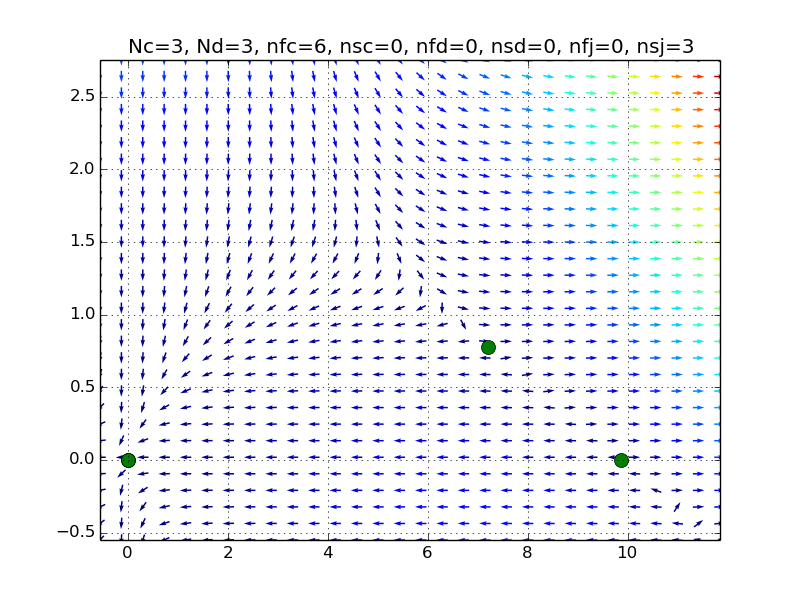
\includegraphics[scale=0.5]{abschnitte/beta_im_R2/fig/flow_example.png}
    \caption{Ein Flussdiagramm für $\beta(\alpha_1,\alpha_2 )$.}
    \label{beta_allgemein:fig:fluss_beispiel}
   \end{figure}


  \subsection{Stabilitätsbedingungen im $\mathbb{R}^2$}
    Für ein System mit zwei Kopplungskonstanten vereinfacht sich die 
    Untersuchung erheblich, da der Phasenraum der $\mathbb{R}^2$ ist und 
    die Stabilitätsmatrix 
    die Form
	\begin{equation}
	 \dbda = \begin{pmatrix}
	          \sum\limits_{i=2,j=0}i \alpha_1^{i-1} \alpha_2^j X^1_{ij} &
	          \sum\limits_{i=2,j=1}j \alpha_1^i \alpha_2^{j-1} X^1_{ij}\\
	          \sum\limits_{i=1,j=2}i \alpha_1^{i-1} \alpha_2^j X^2_{ij} &
	          \sum\limits_{i=0,j=2}j \alpha_1^i \alpha_2^{j-1} X^2_{ij}
	         \end{pmatrix}\label{eq:beta_im_R2:stab_matrix}
	\end{equation}
    annimmt. Die Eigenwerte von $\dbda$ können explizit 
    als\begin{equation}
    \lambda_{+/-}=\frac12 \Sp \pm \sqrt{ \left( \frac{\Sp}{2} \right)^2-\Det } 
    \label{eq:beta_im_R2:lambda}
    \end{equation}
    angegeben werden. Es wird nun kurz begründet, warum ein vollständig 
    wechselwirkender Fixpunkt im allgemeinen als hyperbolisch, d.h. 
    $\Re\lambda_{+/-}\neq 0$, angenommen 
    werden darf, danach wird gezeigt, dass teilweise wechselwirkende Fixpunkte 
    für beliebig hohe Ordnung nicht-hyperbolisch sind. Im $2$-dimensionalen 
    Fall lässt sich jedoch ein alternatives Stabilitätskriterium für solche 
    Fixpunkte finden.
    \subsubsection{hyperbolischer Fixpunkt}
      Sind $\Sp$ und $\Det$ nicht Null, lässt sich das Vorzeichen der 
      Eigenwerte leicht Nachrechnen, das Ergebnis ist in Tabelle 
      \ref{beta_im_R2:tab:stabilitaet_hyperbolisch} zu sehen.
  
      \begin{table}[h]
	\centering
	\begin{tabular}{ccccc}
	\toprule \midrule
	 $\Sp $& $\Det $ & $\Re\lambda_+$ &$\Re\lambda_-$ & UV-Verhalten \\
	 \midrule 
	 $>0$	& $>0$	&$>0$ & $>0$	& repulsiv   \\
	 $<0$	& $>0$	&$<0$ & $<0$	& attraktiv  \\
	  -     & $<0$	&$>0$ & $<0$	& Sattelpunkt\\
	  \midrule
	  \bottomrule
	\end{tabular}
	\caption{Das UV-Verhalten hyperbolischer Fixpunkte für $\Sp\neq0$ 
	und $\Det \neq 0$.}
	\label{beta_im_R2:tab:stabilitaet_hyperbolisch}
\end{table}
      
	An einem vollständig wechselwirkenden Fixpunkt 
	$(\alpha^*_1\neq 0,\alpha_2^*\neq 0)^\text{T}$ sind in der Regel alle 
	Einträge von \eqref{eq:beta_im_R2:stab_matrix} ungleich Null. 
	Die Koeffizienten $X_{ij}^1$ und $X_{ij}^2$ hängen zwar von den gleichen 
	Parametern, der Anzahl und Darstellung der Teilchen und den Eigenschaften der 
	Eichgruppe, ab, es gibt aber keinen Grund, warum $\left.\Det\right|_*=0$ sein 
	sollte. Wenn dies in einer bestimmten Ordnung der Fall ist, sollte zur 
	Untersuchung dieses Fixpunktes die nächst höhere Ordnung Störungstheorie mit 
	berücksichtigt werden, um sinnvolle Aussagen treffen zu können.
      

    \subsubsection{nicht-hyperbolischer Fixpunkt}\label{beta_im_R2:nicht-hyperbolischer_Fixpunkt}
%       In dem Fall, dass bei $\alpha^*$ ein Eigenwert 
%       verschwindet, ist $\left.\Det\right|_*=\lambda_+|_* \lambda_-|_* = 0$ und
%       \begin{alignat}{3}
%       &\left.\lambda_+\right|_* = \left.\Sp\right|_* \quad && \lambda_-|_*=0  
%       \quad && \text{für }\left.\Sp\right|_*\geq 0 \\
%       &\lambda_+|_* = 0   \quad && \lambda_-|_*=\left.\Sp\right|_*  \quad && 
%       \text{für }\left.\Sp\right|_*\leq 0 
%       \quad .
%       \end{alignat}
%       Außerdem 
%       \begin{equation}
% 	\left.\frac{\partial \lambda_{+/-}}{\partial \alpha_i}\right|_*=
% 	\left[-\frac{1}{2} \frac{\partial \Sp}{\partial \alpha_i} 
% 	+ \frac{1}{\lambda_{-/+} }
% 	\frac{\partial \Det}{\partial \alpha_i} \right]_*
% 	\quad ,
%       \end{equation}
%       wobei $\lambda_{+/-}|_*$ der verschwindende Eigenwert ist.
	 Ein teilweise wechselwirkender Fixpunkt, o.E. 
	 $\alpha^*=(\alpha_1^*,0)$,  
	 führt zu der Stabilitätsmatrix 
	 \begin{equation}
	 \dbdafix = \begin{pmatrix}
	          \sum\limits_{i=2}i (\alpha_1^*)^{i-1}  X^1_{i0} &
	          \sum\limits_{i=2} (\alpha_1^*)^i  X^1_{i1}\\
	          0&
	          0
	         \end{pmatrix} \quad . \label{eq:beta_im_R2:stab_matrix_0}
	 \end{equation}
	 mit den Eigenvektoren und Eigenwerten
	 \begin{equation}
	 e_1=\begin{pmatrix}1 \\0 \end{pmatrix} \quad , \quad
	 e_2\propto\begin{pmatrix}
		  -\sum_{i=2} (\alpha_1^*)^i X^1_{i1} 
		   \\
		  \sum_{i=2}i (\alpha_1^*)^{i-1}  X^1_{i0} 
	           \end{pmatrix} \quad , \quad
	 \lambda_1 = \sum_{i=2}i (\alpha_1^*)^{i-1}  X^1_{i0} \quad , \quad
	     \lambda_2=0      \quad .
	 \end{equation}
	Da in $\beta_2$ die Variable $\alpha_2$ in jedem Monom  
	 mindestens zur zweiten Potenz auftaucht, ist dies für 
	 beliebig hohe Ordnung zu erwarten, sodass hier ein alternatives Kriterium 
	 für das UV-Verhalten des Fixpunktes gefunden werden muss.  


	Zunächst wird \eqref{eq:beta_allgemein:beta_linear} um die zweite 
	Ordnung der Taylorentwicklung ergänzt,
     \begin{equation}
     \beta_i(\alpha) \simeq \sum\limits_{m=1}^2 \left. \frac{\partial \beta_i
     }{\partial
      \alpha_m}\right|_* \left(\alpha_m-\alpha^*_m\right) + \frac12 
      \sum\limits_{m,n=1}^2 
       \left(\alpha_m-\alpha^*_m\right)
      \left.\frac{\partial^2 \beta_i}{\partial\alpha_m \partial\alpha_n}
      \right|_* \left(\alpha_n-\alpha^*_n\right) \quad .
      \end{equation}
%      oder in vektorieller Schreibweise in der Basis der Eigenvektoren
%      \begin{equation}
%      \ddt (K_1e_1+K_2e_2)\simeq\dbdafix (K_1e_1+K_2e_2) +
%      (K_1e_1+K_2e_2) \cdot \left.\left(\nabla \dbda \right)\right|_*
%       (K_1e_1+K_2e_2) \quad .
%      \end{equation}
%     Es werden die Ableitungen der Stabilitätsmatrix benötigt
%     \begin{align}
%      \left.\frac{\partial}{\partial \alpha_1} \frac{\partial \beta_i}{\partial 
%      \alpha_n}\right|_* &= \left. 
%      \begin{pmatrix}
% 	\sum\limits_{i=2,j=0} i (i-1) \alpha_1^{i-2}\alpha_2^j X_{ij}^1 &
% 	\sum\limits_{i=2,j=1} ij \alpha_1^{i-1}\alpha_2^{j-1} X_{ij}^1 \\
% 	\sum\limits_{i=2,j=2}i(i-1) \alpha_1^{i-2} \alpha_2^j X_{ij}^2 &
% 	\sum\limits_{i=1,j=2} ij \alpha_1^{i-1}\alpha_2^{j-1} X_{ij}^2
%      \end{pmatrix}_{in} \right|_*   \\
%      &=\begin{pmatrix}
% 	\sum\limits_{i=2} i (i-1) \alpha_1^{i-2} X_{ij}^1 &
% 	\sum\limits_{i=2} i \alpha_1^{i-1} X_{i1}^1 \\
% 	0 &0
%      \end{pmatrix}_{in}
%     \end{align}
%     
%     \begin{align}
%      \left.\frac{\partial}{\partial \alpha_2} \frac{\partial \beta_i}{\partial 
%      \alpha_n}\right|_* &= \left. 
%      \begin{pmatrix}
% 	\sum\limits_{i=2,j=1} i j \alpha_1^{i-1}\alpha_2^{j-1} X_{ij}^1 &
% 	\sum\limits_{i=2,j=2} j(j-1) \alpha_1^{i}\alpha_2^{j-2} X_{ij}^1 \\
% 	\sum\limits_{i=1,j=2}ij \alpha_1^{i-1} \alpha_2^{j-1} X_{ij}^2 &
% 	\sum\limits_{i=1,j=2} j(j-1) \alpha_1^{i}\alpha_2^{j-2} X_{ij}^2
%      \end{pmatrix}_{in} \right|_*   \\
%      &=\begin{pmatrix}
% 	\sum\limits_{i=2} i  \alpha_1^{i-1} X_{i1}^1 &
% 	\sum\limits_{i=2} 2 \alpha_1^{i-1} X_{i2}^1 \\
% 	0 & 
% 	\sum\limits_{i=1} 2 \alpha_1^i X_{i2}^2
%      \end{pmatrix}_{in}
%     \end{align}
    Wie in Abschnitt \ref{beta_allgemein:Verhalten} wird diese Gleichung in 
    der Eigenbasis der Stabilitätsmatrix geschrieben
    \begin{align}
     \dot{K}_1 (t) e_1^i +\dot{K}_2 e_2^i &= \sum\limits_{k,m=1}^2
     K_k(t) \frac{\partial \beta _i}{\partial \alpha_m} e_k^m 
     + \frac12 \sum\limits_{k,l,m,n=1}^2
     K_k(t)K_l(t)\frac{\partial^2 \beta _i}{\partial \alpha_m \alpha_n}e_k^m  
     e_l^n \\
     &= K_1(t)\lambda_1 e_1^i  + \frac12 \sum\limits_{k,l,m,n=1}^2
     K_k(t)K_l(t)\frac{\partial^2 \beta _i}{\partial \alpha_m \alpha_n}e_k^m  
     e_l^n 
     \quad . \label{eq:beta_im_R2:zweite_ordnung}
    \end{align}
    Die Indizes $k$ und $l$ laufen dabei für die zwei Eigenvektoren, während 
    $m$, $n$ und $i$ für die Komponente eines Vektors stehen. Der 
    Koeffizientenvergleich in $e_1$ führt in erster Ordnung zum gleichen 
    Ergebnis wie beim hyperbolischen Fixpunkt. Auf der kritischen Hyperläche 
    gilt demnach $\lambda_1<0 \Rightarrow K_1(t)\rightarrow 0$ für $t$ groß, 
    oder $\lambda>0 \Rightarrow K_1(t)\equiv 0$, da der Fixpunkt sonst nicht 
    erreicht wird. Für große $t$ wird \eqref{eq:beta_im_R2:zweite_ordnung} 
    damit zu 
    \begin{align}
     \dot{K}_2 e_2^i &= \frac{1}{2} K_2(t)^2 \sum\limits_{m,n=1}^2 
     \left.\frac{\partial^2 \beta_i}{\partial \alpha_m \partial \alpha_n}
     \right|_* e_2^m e_2^n
     \\&= \frac12 K_2(t)^2 \sum\limits_{m,n=1}^2 \left[ \left(e_2^m 
     \frac{\partial}{\partial \alpha_m} \right) 
     \left(e_2^n \frac{\partial}{\partial \alpha_n} \right) - e_2^m 
     \frac{\partial e_2^n}{\partial \alpha_m} \frac{\partial}{\partial \alpha_m}
     \right]_* \beta_i \\
     &= \frac12 K_2(t)^2 \left[ \sum\limits_{m=1}^2 e_2^m 
     \frac{\partial\lambda_2}{\partial \alpha_m}e_2^i - \sum\limits_{m,n=1}^2 
     e_2^m \frac{\partial e_2^n}{\partial \alpha_m} 
     \frac{\partial}{\partial \alpha_n} \beta_i \right]_* \quad . 
     \label{eq:beta_im_R2:mischterm}
    \end{align}
    Für $i=2$ kann eine Lösung wie folgt gefunden werden. Der zweite Term in 
    \eqref{eq:beta_im_R2:mischterm} ist wegen 
    \eqref{eq:beta_im_R2:stab_matrix_0} gleich Null.
    Aus \eqref{eq:beta_im_R2:lambda} und \eqref{eq:beta_im_R2:stab_matrix} 
    erhält man am Fixpunkt
    \begin{equation}
     \frac{\partial \lambda_2}{\partial \alpha_q} = 
     \frac{\partial}{\partial \alpha_q} 
     \frac{\partial \beta_2}{\partial \alpha_2} -
     \frac{\partial \beta_1}{\partial \alpha_2} 
     \left(\frac{\partial \beta_2}{\partial \alpha_1} \right)^{-1}
     \frac{\partial}{\partial \alpha_q} 
     \frac{\partial \beta_2}{\partial \alpha_1} \quad 
         \begin{cases}
     =0 \text{ für }q=1\\
     \neq 0 \text{ für }q=2 
   \end{cases}
   \quad .
    \end{equation}
    Es bleibt 
    \begin{equation}
     \dot{K}_2(t) =\frac12 K_2(t)^2  e_2^2 
     \left. \frac{\partial \lambda_2}{\partial \alpha_2} \right|_* \quad 
   \text{mit der Lösung} \quad 
     K_2(t) = \frac{2}{2 K_2(0)^{-1} - 
     e_2^2 \frac{\partial \lambda_2}{\partial \alpha_2}t } \quad .
    \end{equation}
    Da Eigenvektoren nur bis auf ein Vielfaches bestimmt sind, kann 
    $e_2^2>0$ gewählt werden. Damit $\alpha(t=0)$ physikalisch ist folgt 
    $K_2(0)>0$, und damit $K_2(t)$ für steigendes $t$ keinen Pol passiert folgt 
    \begin{equation}
     \frac{\partial \lambda_2}{\partial \alpha_2} < 0
     \label{eq:beta_im_R2:Bedingung}
    \end{equation}
    als Bedingung für einen in $e_2$-Richtung attraktiven Fixpunkt.
    Allgemein ist es nicht möglich, die DGL \eqref{eq:beta_im_R2:mischterm} 
    mit $i=1$ zu lösen, da der zweite Term in der Klammer keine einfachen Eigenschaften 
    aufweist. Da die DGL aber für jedes $i$ einzeln gelten muss, muss jede 
    Lösung mindestens \eqref{eq:beta_im_R2:Bedingung} erfüllen. In der Praxis 
    lässt sich jedoch tatsächlich feststellen, dass 
    \eqref{eq:beta_im_R2:Bedingung} die UV-Stabilität eines Fixpunktes exakt 
    vorhersagt. Daher wird diese Bedingung im Folgenden weiter verwendet.

 